\documentclass[UTF8]{ctexart}
\usepackage{setspace}
\usepackage[letterpaper,top=2cm,bottom=2cm,left=3cm,right=3cm,marginparwidth=1.75cm]{geometry}
\usepackage{listings}
\usepackage{xcolor}      %代码着色宏包

\usepackage{amsmath}
\usepackage{amssymb}\usepackage{mathabx}
\usepackage{amsfonts}
\usepackage{tikz}
\usepackage{verbatim}
\usepackage[mathscr]{eucal}
\usepackage{graphicx}
\usepackage{caption}
\usepackage{subfigure}
\CTEXsetup[format={\Large\bfseries}]{section}

\title{第四次作业}
\author{3200103029 王锦宸}
\date{July 2023}

\begin{document}

\maketitle

此例子给定若干点,使用样条函数进行插值.其中给定点是$(x_i,y_i)$,其中$x_i=i+\sin(i)/2$,$y_i=i+\cos(i^2)$,$i=0,\ldots,9$.
\begin{figure}[h]
    \centering
    \includegraphics[scale=0.5]{interp.eps}
    \caption{插值函数}
    \label{fig:enter-label}
\end{figure}

\end{document}

